
% \clearpage

\vspace{-1mm}
\section{Experiments}
\vspace{-2mm}

This section empirically evaluates our method using the Google Research Football environment (GRF)~\citep{kurach2020google}. We first introduce the experimental settings and then conduct experiments in various difficulties of GRF 11 vs 11 scenarios to compare our method with relevant baselines.

\subsection{Experiment Setups}

\paragraph{Google Research Football}\citep{kurach2020google} is a physics-based 3D football simulator that supports the main football rules such as goals, fouls, corners, penalty kicks, and offside. Google Research Football (GRF) includes a built-in AI bot for the opposing team, whose difficulty can be adjusted between 0 and 1. We define three custom difficulty levels for our experiments on the 11vs11 scenario: easy, medium, and hard. The difficulty levels differ in the bot's reaction time and decision-making defined in GRF, with higher difficulty corresponding to a stronger opponent. The major metric in our experiment is Goal Difference per Match (GDM), calculated as the average number of goals scored in all league matches minus the average number of goals conceded per match. An illustration of the game can be seen in Figure.~\ref{fig:football_main}.  For more details about the GRF implementation, please refer to Appendix~\ref{app:grf}.




\paragraph{Datasets.} We utilize two datasets in our approach. The first is the textbook dataset, which serves as the knowledge base for the \topic~framework. We collect this dataset from the open source book dataset RedPajama-1T~\citep{together2023redpajama}, focusing on titles and abstracts related to football or soccer. After filtering, we obtain a curated set of ninety books closely aligned with the domain. The second dataset is the initial state of our imaginary data generation process. 
We sample 7,500 states from the rollout of a rule-based policy in GRF competing with the hard built-in AI. Due to limited resources, to distill the policy, we imagine 75,000 transitions via \algo, which is 10 times compared to the initial states.

% During the imaginary data generation step, we treat each sampled data point as an initial state and generate $H$ future timesteps using our proposed methodology. This seeding strategy helps ground the imaginary data and improves the overall quality of the generated trajectories.

\paragraph{Baselines.} There are three baselines involved in the experiments. \textbf{LLM-as-agent} directly uses a large language model (GPT 3.5) to output actions conditioned on the current state description. \textbf{LLM-RAG} enhances LLM-as-agent by retrieving relevant knowledge from the database extracted from the tutorial books, similar to the retrieval step in our rehearsing stage, but directly outputs the action without policy learning. \textbf{Rule-based-AI} is a rule-based policy from the Kaggle Football Competition~\citep{anvarov2020football}\footnote{\url{https://github.com/Sarvar-Anvarov/Google-Research-Football}}, which is hand-designed and serves as a reference for the performance of hand-coded policies. \textbf{Random Policy} randomly chooses actions. For the implementation details about the baselines, please refer to Appendix~\ref{app:baseline}.

% \newcolumntype{a}{>{\columncolor{Gray}}c}
\newcolumntype{b}{>{\columncolor{mywhite}}c}


\begin{table*}[t]
\centering
\vspace{-7mm}
\caption{Performance Comparison of Different Policies Against Built-in AI Levels in a GRF 11 vs 11 settings, where the performance of URI is averaged among three different seeds, LLM-as-agent, LLM-RAG is tested with 10 matches, and URI policy and random policy is tested with 40 matches.}
\resizebox{0.85\textwidth}{!}{%
\begin{tabular}{c|c|c|c|c|b||c}
\toprule
\textbf{Level} & & \textbf{LLM-as-agent} & \textbf{LLM-RAG} & \textbf{Random Policy} & \textbf{\algo~(Ours)} & \textbf{Rule-based-AI} \\
\midrule
\multirow{4}{*}{\rotatebox{90}{\textbf{Easy}}} 
& Win & 20\% & 30\% & 2\% & \textbf{37\% $\pm$ 4\%} & 70\% \\
& Draw & 60\% & 60\% & 55\% & 57\% $\pm$ 4\% & 30\% \\
& Lose & 20\% & 10\% & 43\% & 6\% $\pm$ 4\% & 0\% \\
\cmidrule(lr){2-7}
& GDM & 0.0 & 0.2 & -0.58 & \textbf{0.40 $\pm$ 0.14} & 0.7 \\
\midrule
\multirow{4}{*}{\rotatebox{90}{\textbf{Medium}}} 
& Win & 0\% & 20\% & 2\% &  \textbf{42\% $\pm$ 12\%} & 70\% \\
& Draw & 60\% & 60\% & 43\% & 50\% $\pm$ 8\% & 30\% \\
& Lose & 40\% & 20\% & 55\% & 8\% $\pm$ 4\% & 0\% \\
\cmidrule(lr){2-7}
& GDM & -0.4 & 0.0 & -0.76 & \textbf{0.43 $\pm$ 0.24} & 0.7 \\
\midrule
\multirow{4}{*}{\rotatebox{90}{\textbf{Hard}}} 
& Win & 0\% & 0\% & 3\% &  \textbf{32\% $\pm$ 14}\% & 30\% \\
& Draw & 50\% & 40\% & 43\% & 58\% $\pm$ 6\% & 70\% \\
& Lose & 50\% & 60\% & 53\% & 10\% $\pm$ 7\% & 0\% \\
\cmidrule(lr){2-7}
& GDM & -0.5 & -0.6 & -0.73 & \textbf{0.32 $\pm$ 0.14} & 0.3 \\
\midrule
\multirow{2}{*}{\textbf{Average}} & Win & 6.7\% $\pm$ 9.4\% & 16.7\% $\pm$ 12.5\% & 2.3\% $\pm$ 0.5\%& \textbf{40.3\% $\pm$ 6.2\%} & 56\% \\ & GDM & -0.30 $\pm$ 0.22 & -0.13 $\pm$ 0.34 & -0.69 $\pm$ 0.08 & \textbf{0.38 $\pm$ 0.05} & 0.56 \\
\bottomrule
\end{tabular}
}
\label{tab:main_res}
\vspace{-0.5cm}
\end{table*}





\subsection{Policy Performance Compared with Built-in AIs}

 The results in Table \ref{tab:main_res} demonstrate the superiority of the proposed URI approach compared to the baselines in the 11 vs 11 full-game scenarios of the GRF environment. The LLM-based agents, including LLM-as-agent and LLM-RAG, exhibit zero-shot task completion capabilities, outperforming the Random Policy. However, even with the use of RAG techniques, the best-performing LLM-agent can only barely match the performance of the Medium-level built-in AI and fails to achieve any wins against the Hard-level built-in AI. In contrast, URI surpasses the performance of the baseline methods on all difficulty levels. Surprisingly, in the Hard task, URI achieves a higher win rate than the Rule-based Policy. We believe this is due to URI's ability to leverage knowledge from football textbooks and generate high-quality imaginary data for policy learning, enabling it to learn more adaptable and robust policies compared to the hand-crafted Rule-based-AI. These results highlight the effectiveness of the URI in learning strong policies that can handle challenging opponent tasks.





% \begin{table*}[t]
% \centering
% \resizebox{\textwidth}{!}{%
% \begin{tabular}{c|c|c|c|c|c|c|c|c|c|c|c|c}
% \toprule
% & \multicolumn{4}{c|}{11\_vs\_11 (Easy)} & \multicolumn{4}{c|}{11\_vs\_11 (Med)} & \multicolumn{4}{c}{11\_vs\_11 (Hard)} \\
% \midrule
% Method & GDM & Win & Draw & Lose & GDM & Win & Draw & Lose & GDM & Win & Draw & Lose \\
% \midrule
% \cellcolor{mywhite}\algo~(Ours)  & \cellcolor{mywhite} \textbf{0.40 $\pm$ 0.14} & \cellcolor{mywhite} \textbf{37\% $\pm$ 4\%} &\cellcolor{mywhite} 57\% $\pm$ 4\% &\cellcolor{mywhite} 6\% $\pm$ 4\% &\cellcolor{mywhite} \textbf{0.43 $\pm$ 0.24} &\cellcolor{mywhite}42\% $\pm$ 12\% & \cellcolor{mywhite} 50\% $\pm$ 8\% & \cellcolor{mywhite} 8\% $\pm$ 4\% &\cellcolor{mywhite} \textbf{0.32 $\pm$ 0.14} & \cellcolor{mywhite} 32\% $\pm$ 14\% & \cellcolor{mywhite} 58\% $\pm$ 6\% & \cellcolor{mywhite} 10\% $\pm$ 7\% \\
% LLM-as-agent & 0.0 & 20\% & 60\% & 20\% & -0.4 & 0\% & 60\% & 40\% &-0.5 & 0\% & 50\% & 50\% \\
% LLM-RAG & 0.2 & 30\% & 60\% & 10\% &0.0  & 20\% & 60\% & 20\% & -0.6 & 0\% & 40\% & 60\% \\
% Random Policy & -0.58 & 2\% & 55\% & 43\% & -0.76 & 2\% & 43\% & 55\% &-0.73 & 3\% & 43\% & 53\% \\
% \midrule
% Rule-based-AI & 0.7 & 70\% & 30\% & 0\% & 0.7 & 70\% & 30\% & 0\% &0.3 & 30\% & 70\% & 0\% \\
% \bottomrule
% \end{tabular}
% }
% \caption{Performance Comparison of Different Policies Against Built-in AI Levels in a Football Simulator, where the performance of URI is averaged among three different seeds, LLM-as-agent, LLM-RAG is tested with 10 matches, and the random policy is tested with 60 matches.
% % In the game \textbf{11\_vs\_11}, both teams are eleven players, and the difficulties mean the opponent's skill level with the game build-in AI. For more detailed information, please refer to Appendix .\ref{}
% }
% \label{tab:main_res}
% \vspace{-0.5cm}
% \end{table*}




% \begin{table*}[t]
% \centering
% \resizebox{\textwidth}{!}{%
% \begin{tabular}{c|c|c|c|c|c|c|c|c|c|c|c|c}
% \toprule
% & \multicolumn{4}{c|}{11\_vs\_11 (Easy)} & \multicolumn{4}{c|}{11\_vs\_11 (Med)} & \multicolumn{4}{c}{11\_vs\_11 (Hard)} \\
% \midrule
% Method & GDM & Win & Draw & Lose & GDM & Win & Draw & Lose & GDM & Win & Draw & Lose \\
% \midrule
% \addlinespace
% \cellcolor{mywhite}\algo~(Ours)  & \cellcolor{mywhite} \textbf{0.40 $\pm$ 0.14} & \cellcolor{mywhite} \textbf{0.37 $\pm$ 0.04} &\cellcolor{mywhite} 0.57 $\pm$ 0.04 &\cellcolor{mywhite} 0.06 $\pm$ 0.04 &\cellcolor{mywhite} \textbf{0.43 $\pm$ 0.24} &\cellcolor{mywhite}0.42 $\pm$ 0.12 & \cellcolor{mywhite} 0.50 $\pm$ 0.08 & \cellcolor{mywhite} 0.08 $\pm$ 0.04 &\cellcolor{mywhite} \textbf{0.32 $\pm$ 0.14} & \cellcolor{mywhite} 0.32 $\pm$ 0.14 & \cellcolor{mywhite} 0.58 $\pm$ 0.06 & \cellcolor{mywhite} 0.10 $\pm$ 0.07 \\
% \addlinespace\addlinespace
% LLM-as-agent & 0.0 & 0.2 & 0.6 & 0.2 & -0.4 & 0.0 & 0.6 & 0.4 &-0.5 & 0.0 & 0.5 & 0.5 \\
% \addlinespace\addlinespace
% LLM-RAG & 0.2 & 0.3 & 0.6 & 0.1 &0.0  & 0.2 & 0.6 & 0.2 & -0.6 & 0.0 & 0.4 & 0.6 \\
% \addlinespace\addlinespace
% Random Policy & -0.58 & 0.02 & 0.55 & 0.43 & -0.76 & 0.02 & 0.43 & 0.55 &-0.73 & 0.03 & 0.43 & 0.53 \\
% \addlinespace\addlinespace
% \midrule
% \midrule
% % averaged rate\\
% % {'rew': -0.6944444444444445, 'win': 0.022222222222222223, 'draw': 0.47222222222222227, 'lose': 0.5055555555555555, 'replaced_rate': 0.2374343030572211, 'rew_11_vs_11_level_0': -0.5833333333333334, 'win_11_vs_11_level_0': 0.016666666666666666, 'draw_11_vs_11_level_0': 0.55, 'lose_11_vs_11_level_0': 0.43333333333333335, 'replaced_rate_11_vs_11_level_0': 0.23908505440817235, 'rew_11_vs_11_level_1': -0.7666666666666667, 'win_11_vs_11_level_1': 0.016666666666666666, 'draw_11_vs_11_level_1': 0.43333333333333335, 'lose_11_vs_11_level_1': 0.55, 'replaced_rate_11_vs_11_level_1': 0.22922496113701973, 'rew_11_vs_11_level_2': -0.7333333333333333, 'win_11_vs_11_level_2': 0.03333333333333333, 'draw_11_vs_11_level_2': 0.43333333333333335, 'lose_11_vs_11_level_2': 0.5333333333333333, 'replaced_rate_11_vs_11_level_2': 0.2439928936264712}
% Rule-based-AI & 0.7 & 0.7 & 0.3 & 0.0 & 0.7 & 0.7 & 0.3 & 0.0 &0.3 & 0.3 & 0.7 & 0.0 \\
% \bottomrule
% \end{tabular}
% }
% \caption{Performance Comparison of Different Policies Against Built-in AI Levels in a GFootball Simulator, where the performance of URI is averaged among three different seeds, LLM-as-agent, LLM-RAG is tested with 10 matches, and the random policy is tested with 60 matches.
% % In the game \textbf{11\_vs\_11}, both teams are eleven players, and the difficulties mean the opponent's skill level with the game build-in AI. For more detailed information, please refer to Appendix .\ref{}
% }
% \label{tab:main_res}
% \vspace{-0.5cm}
% \end{table*}

% The main result is shown in Table.\ref{tab:main_res}. 1. 首先我们看到,所有的基线的效果都优于random策略,说明基于LLM的agent是具有zero-shot的完成该任务的能力的;但是,即使是使用了RAG技术的LLM-agent,最好也只能勉强和Medium-level的builtinAI持平,在Hard难度上完全无法取胜。
% 2. 相比之下,Uri是唯一一个能够战胜所有level的AI的方法,且其GDM也显著超过了基线的最好水平,


% \begin{table*}[t]
%     \centering
%     \resizebox{\textwidth}{!}{%
%     \begin{tabular}{c|c|c|c|c|c|c|c|c|c|c|c|c|c|c|c|c}
%     \toprule
%          &  \multicolumn{4}{c|}{\algo} & \multicolumn{4}{c|}{LLM-as-agent}  & \multicolumn{4}{c|}{LLM-RAG} & \multicolumn{4}{c}{Rule-based-AI} \\
%          \midrule
%         %    & \multicolumn{3}{c|}{Mean (Mid/Left/Right)}  & \multicolumn{3}{c|}{Mean (Mid/Left/Right)}  & \multicolumn{3}{c|}{Mean (Mid/Left/Right)}  & \multicolumn{3}{c}{Mean (Mid/Left/Right)}  \\  
%         % \midrule
%          % 11\_vs\_1 (Easy)  & \multicolumn{3}{c|}{11111} & \multicolumn{3}{c|}{11111} & \multicolumn{3}{c|}{11111} & \multicolumn{3}{c}{0.53~(0.93/0.36/0.30)} \\  
%          % 11\_vs\_1 (Med)  & \multicolumn{3}{c|}{11111} & \multicolumn{3}{c|}{11111} & \multicolumn{3}{c|}{11111} & \multicolumn{3}{c}{0.41~(0.75/0.28/0.25)} \\  
%          % 11\_vs\_1 (Hard)  & \multicolumn{3}{c|}{11111} & \multicolumn{3}{c|}{11111} & \multicolumn{3}{c|}{11111} & \multicolumn{3}{c}{0.39~(0.72/0.29/0.17)} \\  
%          \midrule
%          Task & GDM & Win & Draw & Lose & GDM & Win & Draw & Lose& GDM & Win & Draw & Lose& GDM & Win & Draw & Lose\\
%          \midrule
%          11\_vs\_11 (Easy) & 0.40 $\pm$ 0.14 & 0.37 $\pm$ 0.04 & 0.57 & 0.06 & &  0.2 & 0.6 &  0.2 & &  0.3 & 0.6 & 0.1 &  & 0.7 & 0.3 & 0.0\\
%          11\_vs\_11 (Med) & 0.43 $\pm$ 0.24  & 0.42 & 0.50 & 0.08 & 0.0 & 0.6 & 0.4 & 0.2 & 0.6 & 0.2 & 0.7 & 0.3 & 0.0 \\
%          11\_vs\_11 (Hard) & 0.32 $\pm$ 0.14 & 0.32 & 0.58 & 0.10 &  0.0 & 0.5 &  0.5& 0.0 & 0.4 & 0.6 & 0.3 & 0.7 & 0.0 \\
%         \midrule
%         \midrule
%         averaged rate\\
%         \bottomrule
%     \end{tabular}
%     }
%     \caption{Performance Comparison of Different Policies Against Built-in AI Levels in a Football Simulator. GDM is an abbreviation of Goal Difference per Match, which is calculated as the average number of goals scored in all league matches minus the average number of goals conceded per match.
%     % In the game \textbf{11\_vs\_1}, our team have eleven players, and the opponent team has only one goalkeeper. It includes three types of difficulty, showing the distance from the goalkeeper from near to far. Each type of map provides attack tests from centre, left, and right, the ball will therefore appear in the corresponding direction according to the test, the test is one-time, if the goal is +1, other situations (such as not kicking in, going out of bounds, being guarded by the goalkeeper, etc.) are 0.  
%     % In the game \textbf{11\_vs\_11}, both teams are eleven players, and the difficulties mean the opponent's skill level with the game build-in AI. For more detailed information, please refer to Appendix .\ref{}
%     }
%     \label{tab:main_res}
% \end{table*}






% \begin{itemize}
%     \item discussion on results
%     \item capabilities graph [ziyan] [lp]
% \end{itemize}
% In this section, we present a comprehensive benchmark of various policy algorithms against built-in AI agents across multiple levels of complexity. The evaluation metrics include win, draw, and loss rates, offering a holistic view of each algorithm's performance. The benchmarked algorithms include Policy Learning via Reading (PER),  and traditional Rule-based AI. These were tested across five distinct levels, escalating in difficulty, to ascertain their adaptability and learning efficiency in diverse environments. An aggregated rate across all levels is provided to summarize overall performance.


% In evaluating the effectiveness of our proposed LLM-based methodologies, we conducted a series of benchmark tests against various built-in AI levels in a simulated football environment. The following table presents the performance metrics of different policy implementations, including Large Language Models as agents (LLM-as-agent), Large Language Models with planning capabilities (LLM-planning), Large Language Models using Retrieval-Augmented Generation (LLM-RAG), and traditional Rule-based AI. The metrics used are the winning, drawing, and losing rates against built-in AI opponents across five difficulty levels.




% The benchmark results provide compelling evidence that PER outperforms other algorithms, including various configurations of Large Language Models (LLMs) and traditional Rule-based AI, across multiple complexity levels. The superiority of PER is evident in several key aspects:

% \textbf{Consistency Across Levels:} PER demonstrates remarkable consistency in its performance, maintaining a high win rate and a low loss rate across all levels. This is indicative of its robustness and adaptability to varying challenges, a critical attribute for AI algorithms in dynamic environments.


% \textbf{Superiority in Complex Scenarios:} At higher levels, where the complexity and the requirement for strategic depth increase, PER's advantage becomes even more pronounced. Its capability to handle intricate scenarios effectively underscores its advanced learning and decision-making mechanisms.

% \textbf{Resilience Against Rule-based AI:} In direct comparisons with Rule-based AI, PER not only outperforms but also demonstrates a clear understanding of the rule-based agent's strategy, effectively countering it. This resilience highlights PER's strength in adapting to and overcoming structured, predictable strategies.

% In summary, the aggregated data unequivocally suggests that Priority Experience Replay stands out as the superior algorithm in this benchmark. Its consistent performance, learning efficiency, balanced strategy, proficiency in complex scenarios, and resilience against rule-based strategies underscore its potential as a leading approach in reinforcement learning.



\subsection{Effectiveness of Code Extraction and Aggregation}

\begin{wrapfigure}[9]{r}{0.4\textwidth}
\vspace{-1.7cm}
    \begin{center}
        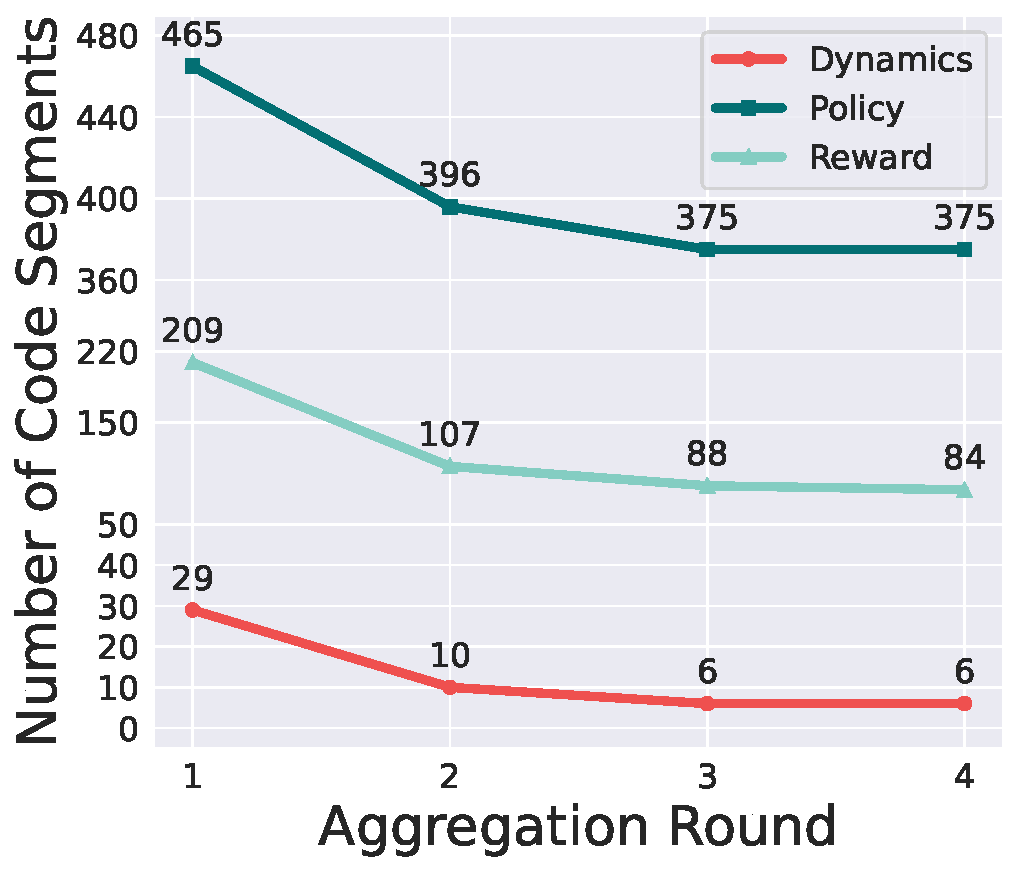
\includegraphics[width=0.85\linewidth]{fig/code_segment_reduction_aggregation.pdf}
        \caption{Knowledge Segment Aggregation.}
        \label{fig:code_segment}
    \end{center}
    \vspace{-3.6cm}
\end{wrapfigure}
According to Section.~\ref{sec:book_content_understanding}, we perform an iterative process of code extraction and aggregation to understand the football textbooks and obtain executable knowledge. Figure.~\ref{fig:code_segment} shows the reduction in the number of code segments for dynamics, policy, and reward functions over the aggregation rounds. Through iterative aggregation, the number of code segments decreases significantly, which helps condense the extracted knowledge into a more compact and coherent form. 

% In addition, we observe that as the number of aggregation rounds increases, the length of the code segment contents also grows, which can be found in the examples and details provided in the Appendix~\ref{app:code_aggregation}.



% What are the results of code extraction: 
% \begin{itemize}
%     \item shows the number of codes of different functions.
%     \item show examples.
% \end{itemize}

% Show the reduction progress of code aggregation.
% \begin{itemize}
%     \item iteration and number of code.
%     \item example of final results.
% \end{itemize}



% \begin{figure}
%     \vspace{-3em}
%     \centering
%     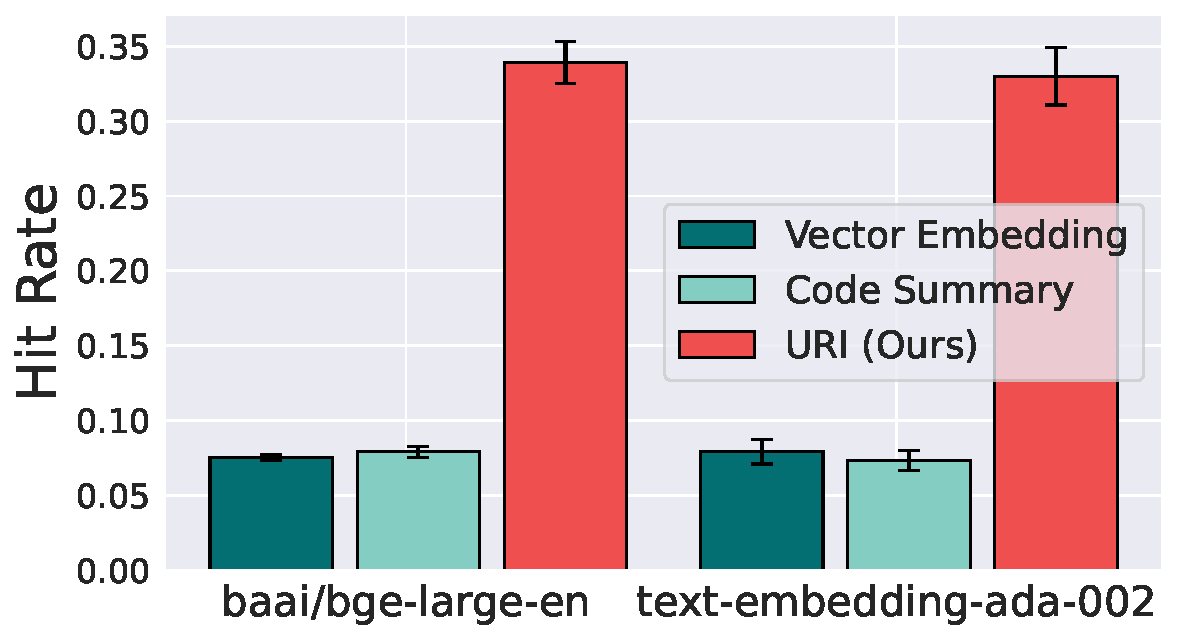
\includegraphics[width=0.4\linewidth]{fig/hitrate.pdf}
%     \hspace{10mm}
%     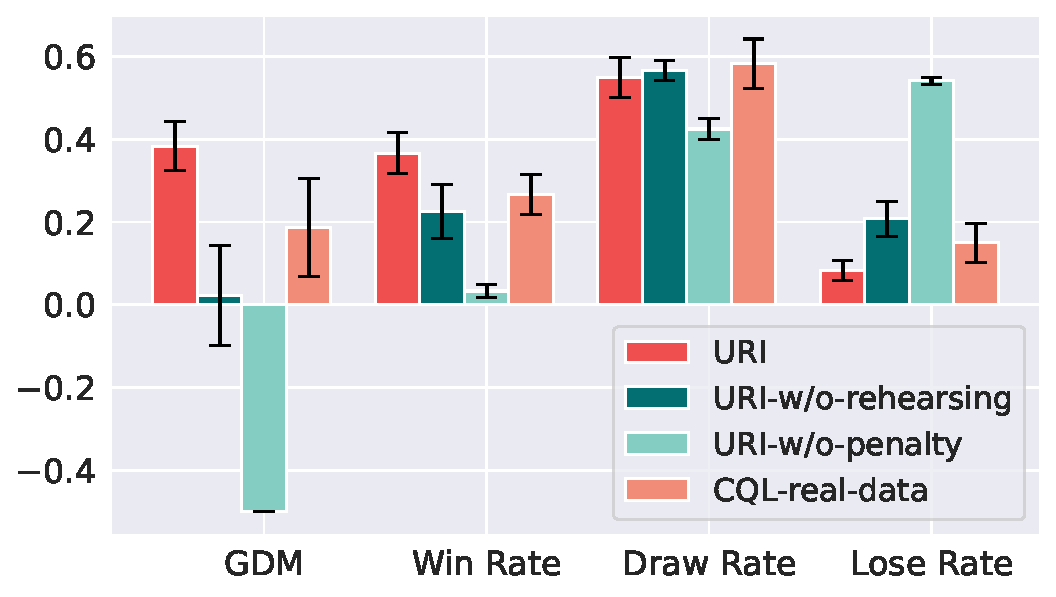
\includegraphics[width=0.4\linewidth]{fig/exp/first_version.pdf}
%     \caption{(a).~Comparison of different code retrieval methods on two pre-trained language models. (b).~Performance comparison of different URI framework variants in the GRF. This figure illustrates the win, draw, and lose rates of the four configurations. The error bars in the figure indicate the standard deviation from the mean performance for each configuration in three random seeds.}
%     \label{fig:hitrate}
%     \vspace{-0.5cm}
% \end{figure}




% \begin{figure}
% \vspace{-3em}
% \centering
% \begin{subfigure}{0.4\linewidth}
% \centering
% 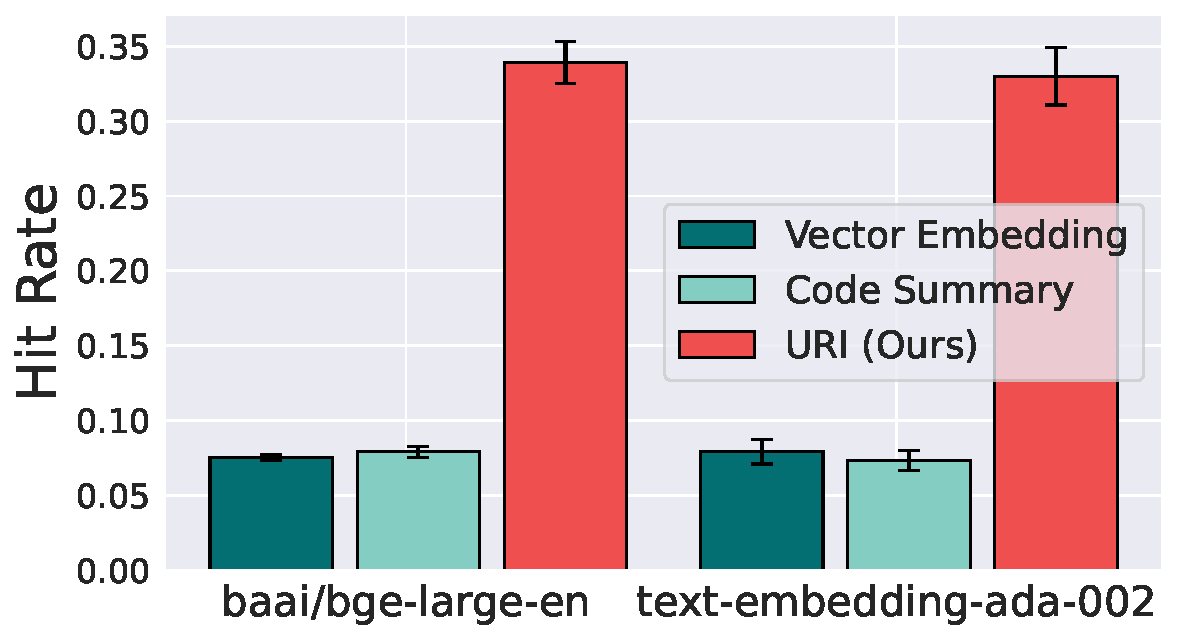
\includegraphics[width=\linewidth]{fig/hitrate.pdf}
% \caption{}
% \label{fig:hitrate_a}
% \end{subfigure}
% \hspace{10mm}
% \begin{subfigure}{0.4\linewidth}
% \centering
% 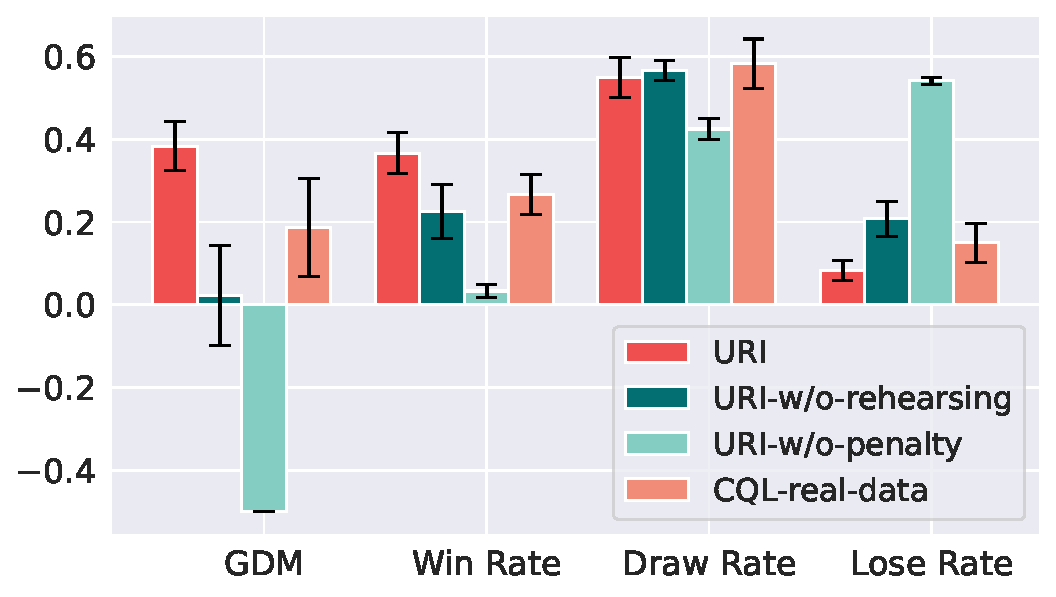
\includegraphics[width=\linewidth]{fig/exp/first_version.pdf}
% \caption{}
% \label{fig:hitrate_b}
% \end{subfigure}

% \caption{(a).~Comparison of different code retrieval methods on two pre-trained language models. (b).~Performance comparison of different URI framework variants in the GRF. This figure illustrates the win, draw, and lose rates of the four configurations. The error bars in the figure indicate the standard deviation from the mean performance for each configuration in three random seeds.}
% \label{fig:hitrate}
% \vspace{-0.5cm}
% \end{figure}



\subsection{Correlation between Knowledge Embedding and Current State Embedding}
\label{exp:emb}

% \begin{wrapfigure}[16]{l}{0.40\textwidth}
% \vspace{-0.3cm}
%     \begin{center}
%         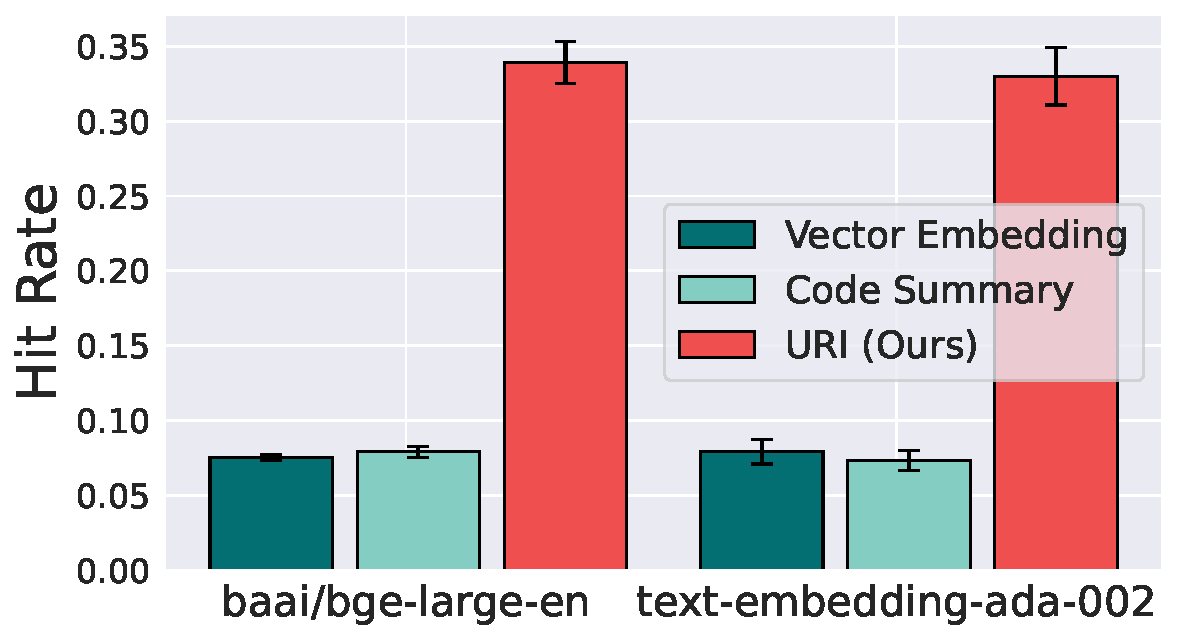
\includegraphics[width=\linewidth]{fig/hitrate.pdf}
%         \caption{Comparison of different code retrieval methods on two pre-trained language models.}
%         \label{fig:hitrate}
%     \end{center}
% \end{wrapfigure}

% In Section.~\ref{sec:sbksr}, we discussed the importance of retrieving relevant code segments based on the current state for effective knowledge instantiation in our PLfB framework. Standard RAG techniques, which directly compare the embeddings of the query (current state) and the documents (code segments), may not work well in this scenario due to the modality gap between the state description and the code content. To address this issue, we proposed the 'obs\_matching' method, which learns a dedicated matcher to score the relevance between the state and the code segments. This matcher is trained to bridge the modality gap and improve the correlation between the state embedding and the code embedding.

To validate the effectiveness of our code embedding method mentioned in Section.~\ref{sec:sbksr}, we conducted experiments comparing it with two baselines: \textbf{Vector Embedding}, which directly compares the state and code embeddings, and \textbf{Code Summary}, which first summarizes the code segments before comparing the embeddings. We evaluate the top-15 hit rate in a hand-crafted test dataset. The observations and actions in the dataset we used are collected by the rule-based policy interacting with the real environment, while the ground-truth codes are labeled by GPT and aggregated using a similar way as in Section.~\ref{sec:book_content_understanding}.
As shown in Figure.~\ref{fig:hitrate}(a), our method significantly outperforms the other two baselines on both pre-trained language models. The hit rate, which measures the proportion of relevant code segments retrieved, is consistently higher for URI across all three random seeds, demonstrating its robustness and superiority in improving the correlation between the state embedding and the code embedding. These results highlight the importance of learning a dedicated matcher for effective code retrieval in our framework. 


% This section examines the interplay between code embedding and current state embedding in our Policy Learning via Reading (PER) framework, with a specific focus on the impact of fine-tuning on code retrieval effectiveness. Understanding this relationship is critical for optimizing the agent's performance in extracting and utilizing knowledge from textual sources for decision-making in a simulated football environment.

% \begin{figure}[ht]
% \centering
% \includegraphics[width=0.75\linewidth]{code_state_embedding_correlation.png}
% \caption{Illustration of the correlation between code embedding and current state embedding before and after fine-tuning in the PER methodology.}
% \label{fig:code_state_embedding}
% \end{figure}

% To demonstrate the capacity of our system to retrieve effective information from code, we compare the results before and after fine-tuning. Metrics such as accuracy or correctness in code retrieval can be used to quantify this impact. Figure.~\ref{fig:code_state_embedding} showcases that fine-tuning significantly enhances the alignment between code embedding and the current state embedding, indicating more accurate and relevant information retrieval post-fine-tuning.

% \begin{figure}[ht]
% \centering
% 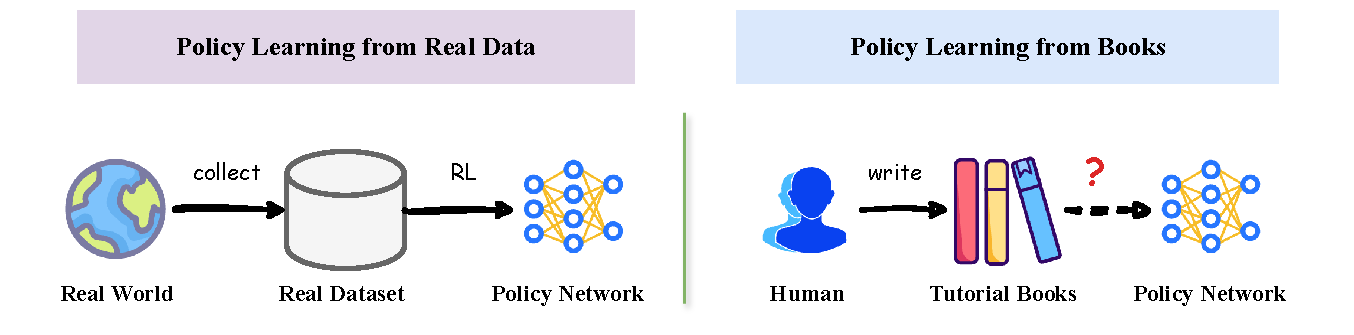
\includegraphics[width=0.75\linewidth]{fig/PER-problem.pdf}
% \caption{Example.}
% \label{fig:code_state_embedding}
% \end{figure}

 % Examining specific instances of code retrieval before and after the fine-tuning process provides practical insights. Initially, the retrieved codes may only partially align with the current state requirements, reflecting a generalized understanding. Post-fine-tuning, the codes demonstrate a high degree of specificity and relevance, indicating a more nuanced understanding and application of football strategies and tactics as per the current game state.
 
% \textbf{[level 2] Comparing Different Fine-Tuning Techniques:} Different fine-tuning techniques can yield varied results in terms of code retrieval efficiency and accuracy. By comparing techniques such as supervised fine-tuning, unsupervised fine-tuning, and reinforcement learning-based fine-tuning, we can determine the most effective method for aligning code and state embeddings in our PER framework. This analysis not only enhances the performance of the agent but also contributes to the broader understanding of fine-tuning impacts in language model-based learning systems.
% \begin{wrapfigure}[18]{r}{0.5\textwidth}
% \vspace{-1cm}
%     \begin{center}
%         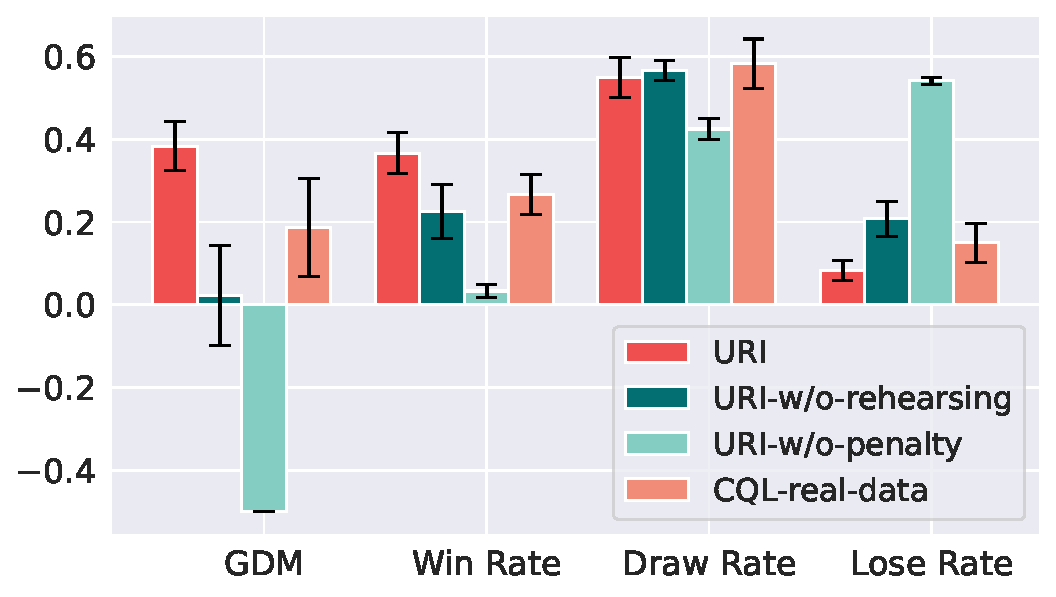
\includegraphics[width=\linewidth]{fig/exp/first_version.pdf}
%         \caption{Performance comparison of different URI framework variants in the GRF. This figure illustrates the win, draw, and lose rates of four configurations. The error bars in the figure indicate the standard deviation from the mean performance for each configuration in three random seeds.}
%         \label{fig:ablation}
%     \end{center}
% \vspace{-0.6cm}
% \end{wrapfigure}


\begin{figure}[t]

\centering
\vspace{-7mm}
\begin{tabular}{cc}
    \subfigure[]{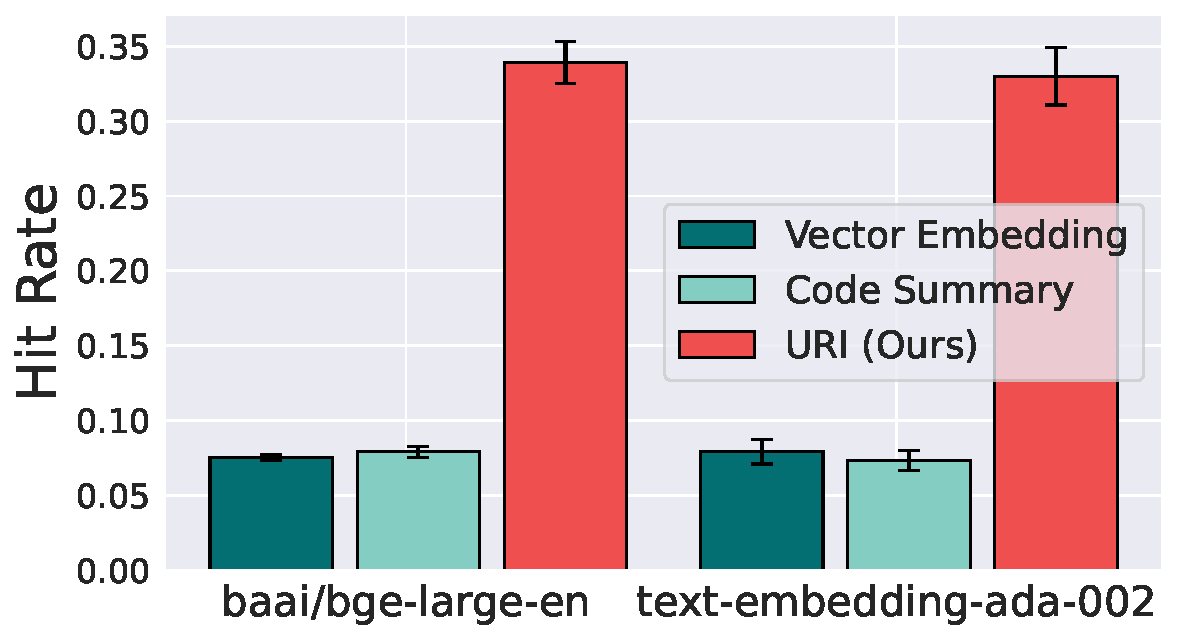
\includegraphics[width=0.45\linewidth]{fig/hitrate.pdf}} 
    \hspace{5mm}
    \subfigure[]{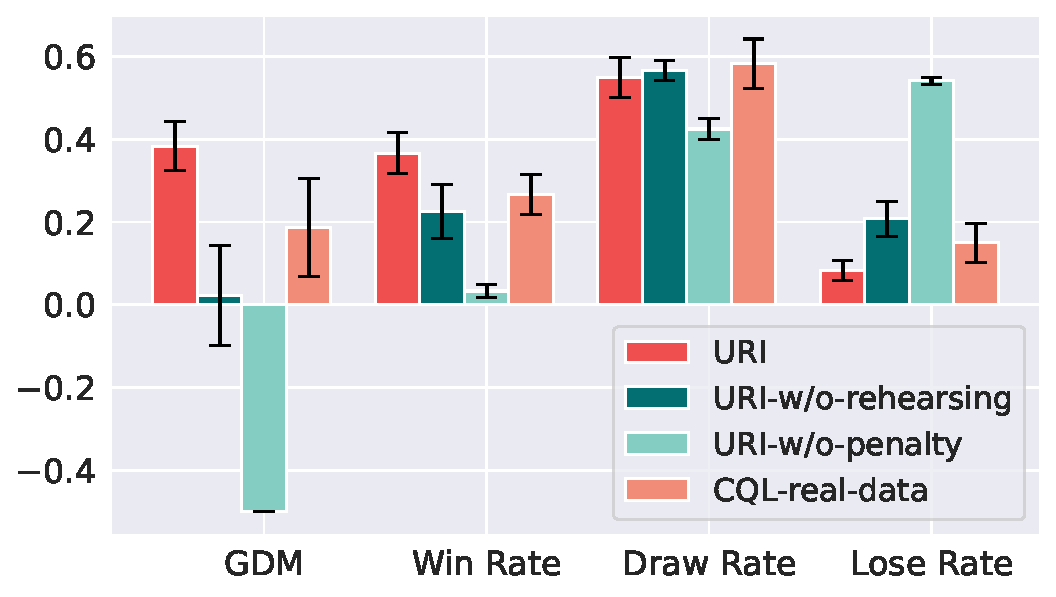
\includegraphics[width=0.45\linewidth]{fig/exp/first_version.pdf}} 
\end{tabular}
\caption{(a).~Comparison of different code retrieval methods on two pre-trained language models. (b).~Performance comparison of different variants of the URI framework in the GRF. This figure illustrates the average GDM, win, draw, and lose rates among the three levels of built-in AIs. The error bars in the figure indicate the standard deviation from the mean performance for each configuration in three random seeds.}
\label{fig:hitrate}
\vspace{-0.5cm}
\end{figure}



\subsection{Tracing the Data Generation Process}

\begin{figure}[h]
    % \centering
    \hspace{-9mm}
    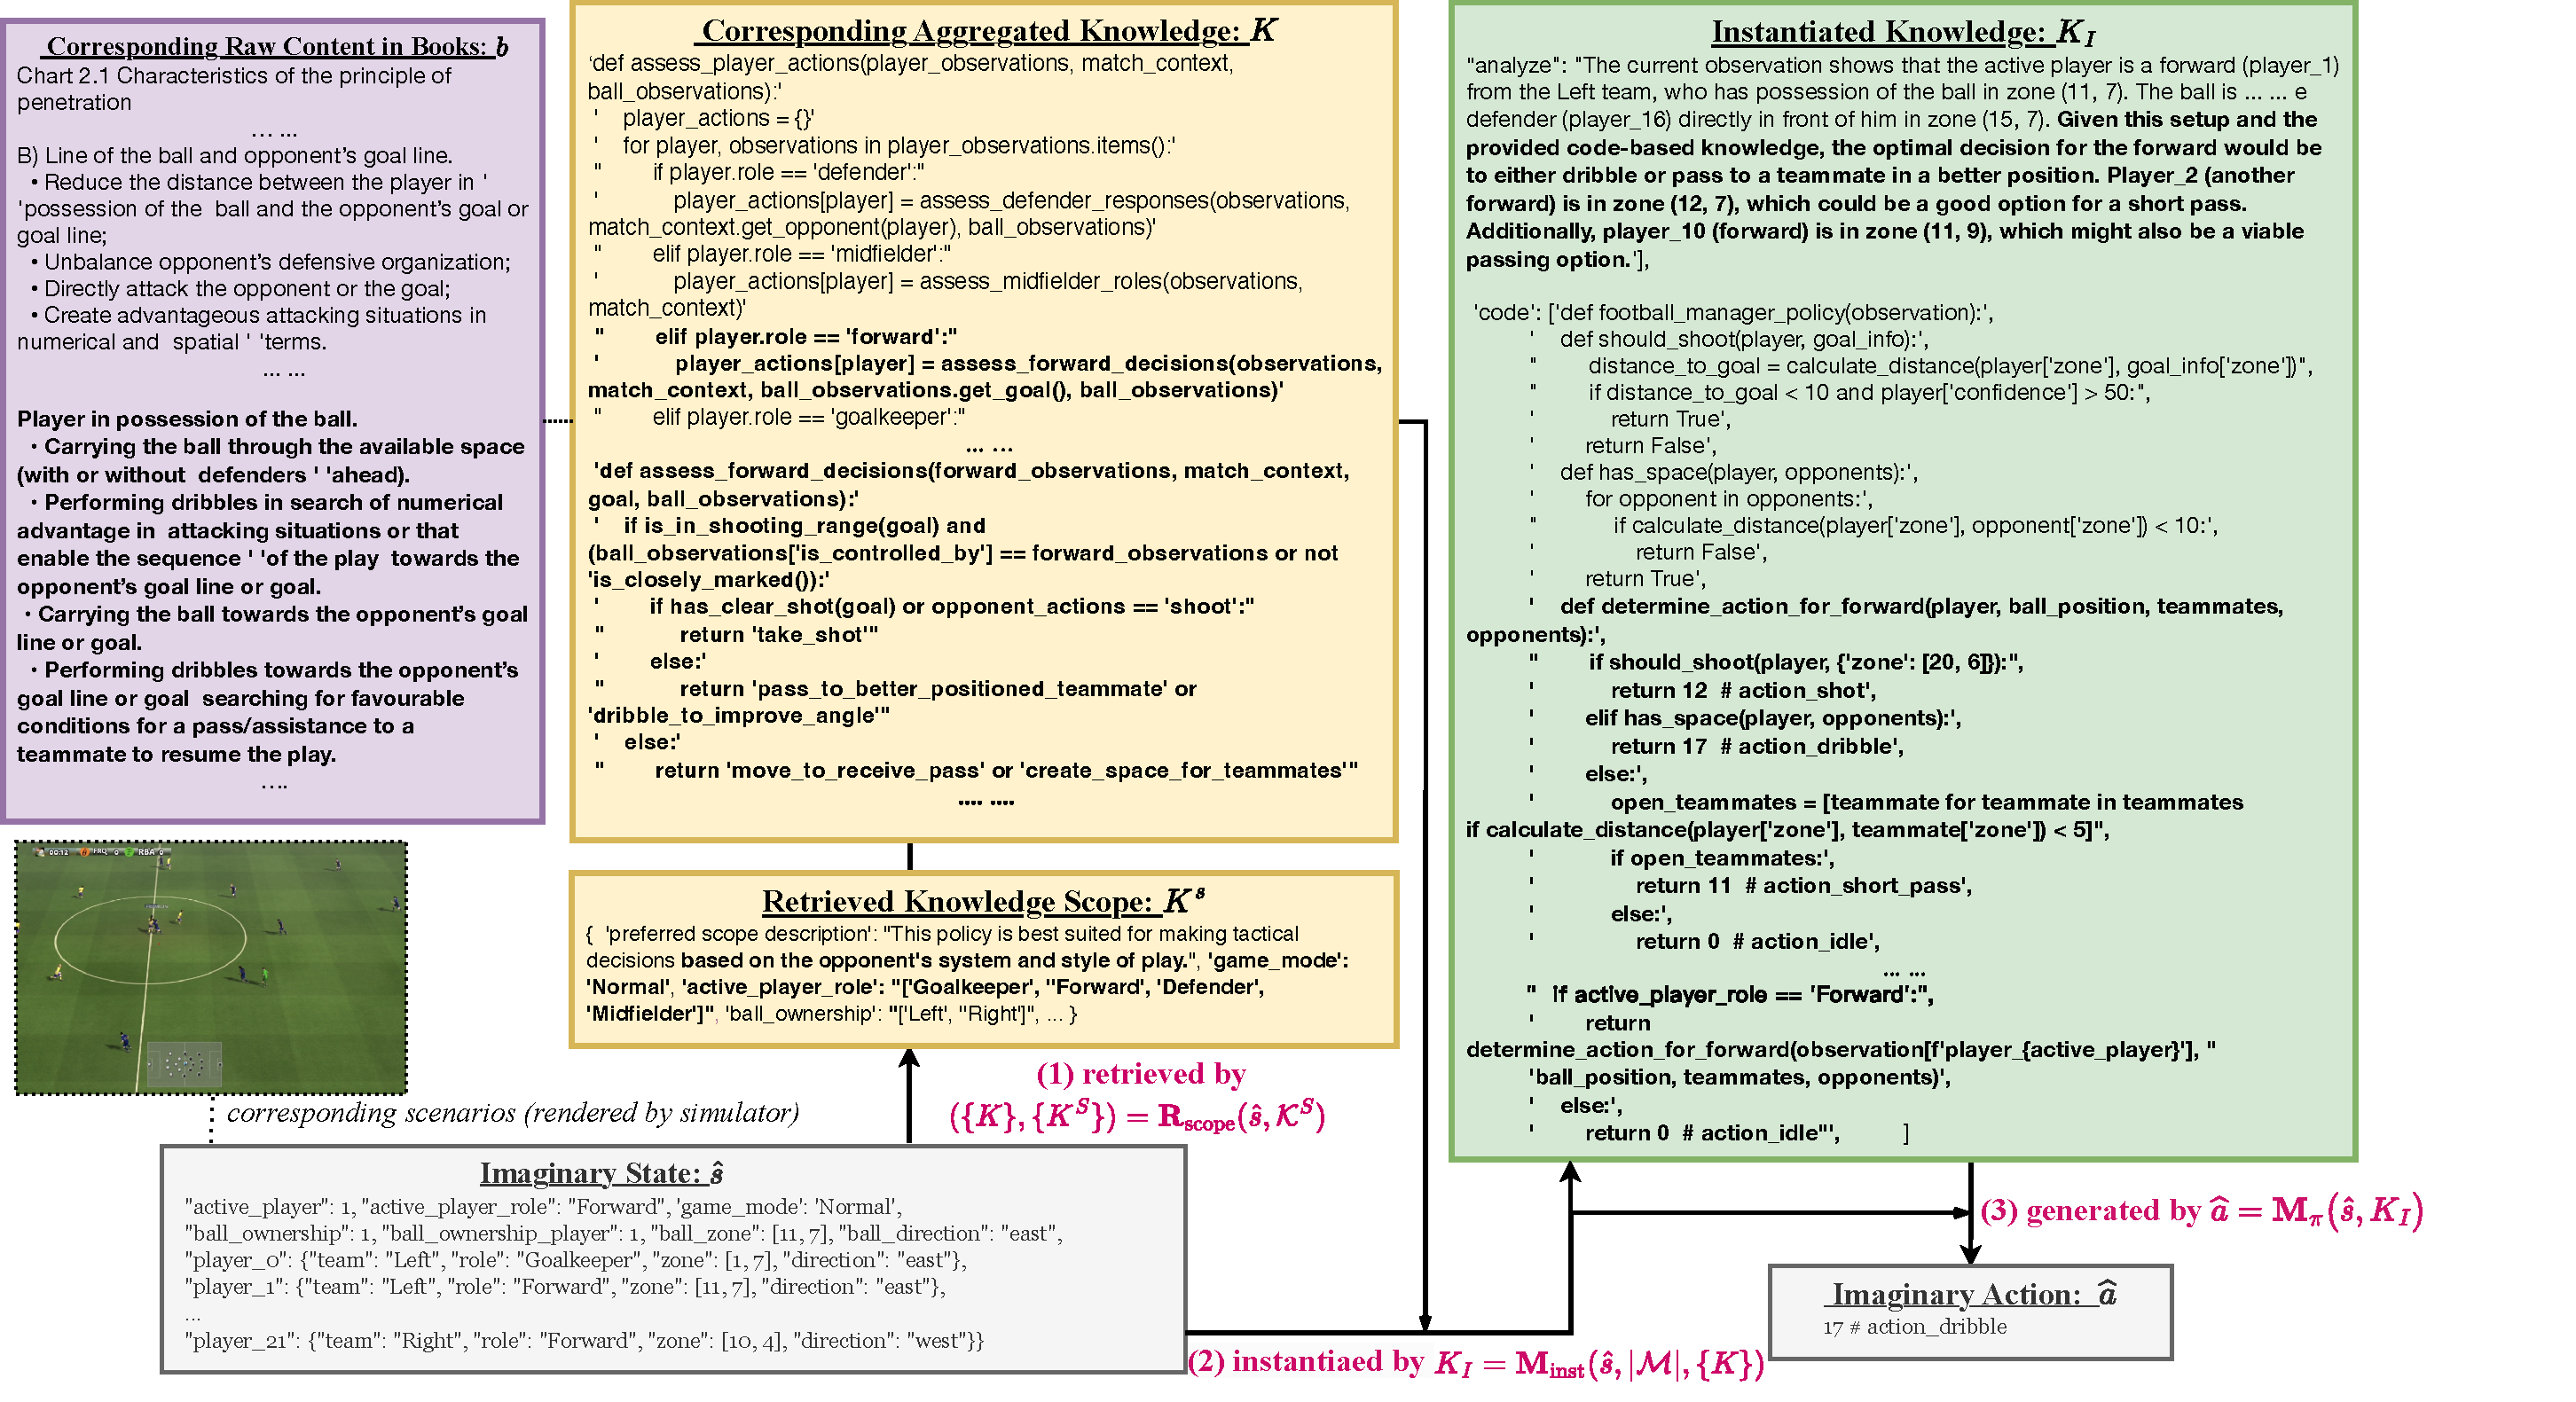
\includegraphics[width=1.2\textwidth]{fig/example2.pdf}
    \caption{Results of the imaginary action generation process. The imaginary state $\hat s$ is collected from the real environment, which is the 12 timestep of a football game, while the rendered image is the corresponding scenario generated by the simulator. The imaginary action is ``dribble'', where the logic is supported by the ``has\_space'' branch in $K_I$. Based on this, we \textbf{bold} the relevant information in the predecessor nodes and skip irrelevant information with the ellipsis ``... ...''.}
    \label{fig:data_gen_demo}
    \vspace{-1mm}
\end{figure}
In \algo, it is crucial to guarantee that the imaginary data include states, actions, and rewards. The task is non-trivial since it has to involve several transformations to align the gap between textual contents in books and decision-making trajectories in MDP. To verify the effectiveness of the data generation process, we trace how $\llm_\pi$ outputs an imaginary action $\hat a$ on an imaginary state $\hat s$, which is actually collected at the start of a football game in GRF. We record all the intermediate outputs to trace the action generation process. The result is shown in Figure.~\ref{fig:data_gen_demo}.   It is clearly shown that the output action ``dribble'' is fully supported by the logic in``has\_space'' branch in $K_I$, ``assess\_forward\_decisions'' function in $K$, and the paragraph of ``Player in possession of the ball'' in the raw content of tutorial books. However, we would like to point out that there are also some examples that demonstrate LLMs having hallucinations in generation, and the retrieved module might also miss the ground-truth piece of knowledge. More results are provided in Appendix~\ref{app:example}. These results indicate the necessity of introspecting in \algo. The relevant ablation studies are in Section.~\ref{exp:abl}.
% 有效的
% 局限性
% 更多的结果


\vspace{-1mm}
\subsection{Importance of the components in URI}
\label{exp:abl}
% \vspace{-2mm}
% \begin{figure}[h]
% \centering
% 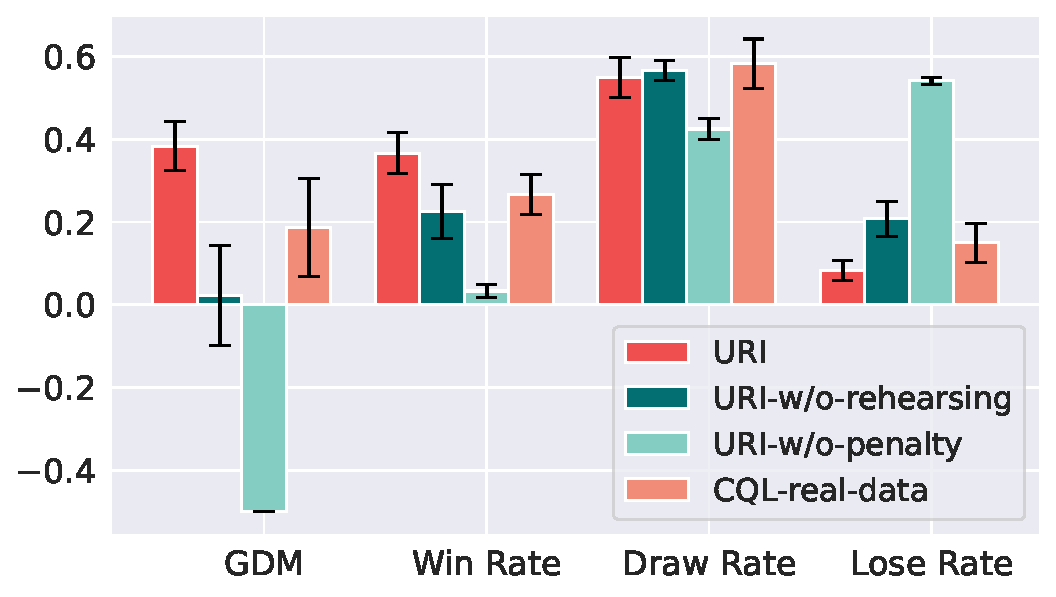
\includegraphics[width=0.7\linewidth]{fig/exp/first_version.pdf}
% \caption{}
% \label{fig:ablation}
% \end{figure}

In this section, we validate the effectiveness of the rehearsing technique presented in Section~\ref{sec:rehearsing} and the CIQL method introduced in Section~\ref{sec:introspecting} through ablation studies. Specifically, we constructed the following variants of the URI framework: (1) \textbf{URI-w/o-rehearsing}, which solves the policy without using the rehearsing dataset and relies on a pre-collected dataset of 7,500 samples for offline RL policy training; (2) \textbf{URI-w/o-penalty}, where penalties  $\eta_\transf$ and $\eta_\rewf$ are zero, same as the standard CQL for policy learning; (3) \textbf{CQL-real-data}, where we collect real data of equivalent scale to the rehearsing-generated data using rule-based AI and apply standard CQL for offline RL policy training. The results are shown in Figure.~\ref{fig:hitrate}(b).

Firstly, URI-w/o-rehearsing demonstrates that without generating a substantial amount of imaginary data through rehearsing, solely relying on offline RL algorithms to train a policy with our pre-collected 7,500 samples is ineffective. The results indicate that it cannot even beat the AI on Easy difficulty, though it still performs better than a random strategy. URI-w/o-penalty underscores the importance of penalizing the uncertain aspects of the outcomes generated from the imaginary data. Neglecting this penalty leads to results worse than those of URI-w/o-rehearsing. 
Finally, our method slightly outperforms CQL-real-data. We attribute this improvement to the strategies inferred from prior knowledge by LLMs, which are partially superior to built-in AI behaviors, or possibly because LLMs generate more diverse data. This illustrates the considerable potential of \topic.


% ablation studies among different components in offline RL.
% \begin{itemize}
%     \item without uncertainty estimator
%     \item without imaginary data.
%     \item different hp-parameters selection [lp].
% \end{itemize}

% \subsection{Ablation studies [ziyan-baseline]}

% [figure]

% \begin{itemize}
%     \item PER
%     \item without-RL: book-rag-$\pi$ [done]
%     \item  without-book-information: GPT-imgdata-$\pi$ [lp]
% \end{itemize}
\vspace{-1mm}
\subsection{Efficiency in inference}
% \vspace{-2mm}
% Table \ref{tab:inference_time} compares the inference time per action for different methods. Our URI approach takes only 0.50 seconds on average to choose an action, which is significantly faster than using LLMs directly as agents (2.84 seconds) or with retrieval-augmented generation (RAG) (4.12 seconds). This makes URI more suitable for real-time decision making in the football simulator. The efficiency gain comes from the fact that URI distills the knowledge from the LLM into a compact policy network, which can be executed quickly without the need for expensive LLM inference at each step.



\begin{wrapfigure}[7]{r}{0.41\textwidth}
\centering
\vspace{-1cm}
\begin{minipage}{0.41\textwidth}
\begin{table}[H]
\caption{Comparison of inference time per action for different methods.}
\centering
\begin{tabular}{ll}
\hline
           & Time Cost(s)
                  \\ \hline


LLM-as-Agent  & 2.84 $\pm$ 0.71  \\

LLM-RAG & 4.12 $\pm$1.46 \\

URI & \textbf{0.009 $\pm$ 0.0004} \\
\hline
\end{tabular}
\vspace{-2cm}
\label{tab:inference_time}
\end{table}
\end{minipage}
\end{wrapfigure}

In real-time decision-making tasks such as playing football, the efficiency of the policy is crucial. We compare the inference time per action for different methods in Table \ref{tab:inference_time}. Our approach takes only 0.009 seconds on average to choose an action, which is significantly faster \textbf{at least 300 times} than using LLMs directly as agents (2.84 seconds) or with retrieval-augmented generation (RAG) (4.12 seconds). This makes URI more suitable for real-time decision-making in the football simulator. The efficiency gain comes from the fact that URI distills the knowledge from the LLM into a compact policy network, which can be executed quickly without the need for expensive LLM inference at each step.


% \subsection{Amount of Imaginary Dataset Used}

% % [figure]

% Show the relationship between the amount of offline dataset used, the imaginary dataset used, and the performance of the learned policy.


\vspace{-1mm}
\subsection{Imaginary Dataset Visualization}  
\begin{wrapfigure}[14]{r}{0.35\textwidth}
\vspace{-0.7cm}
    \begin{center}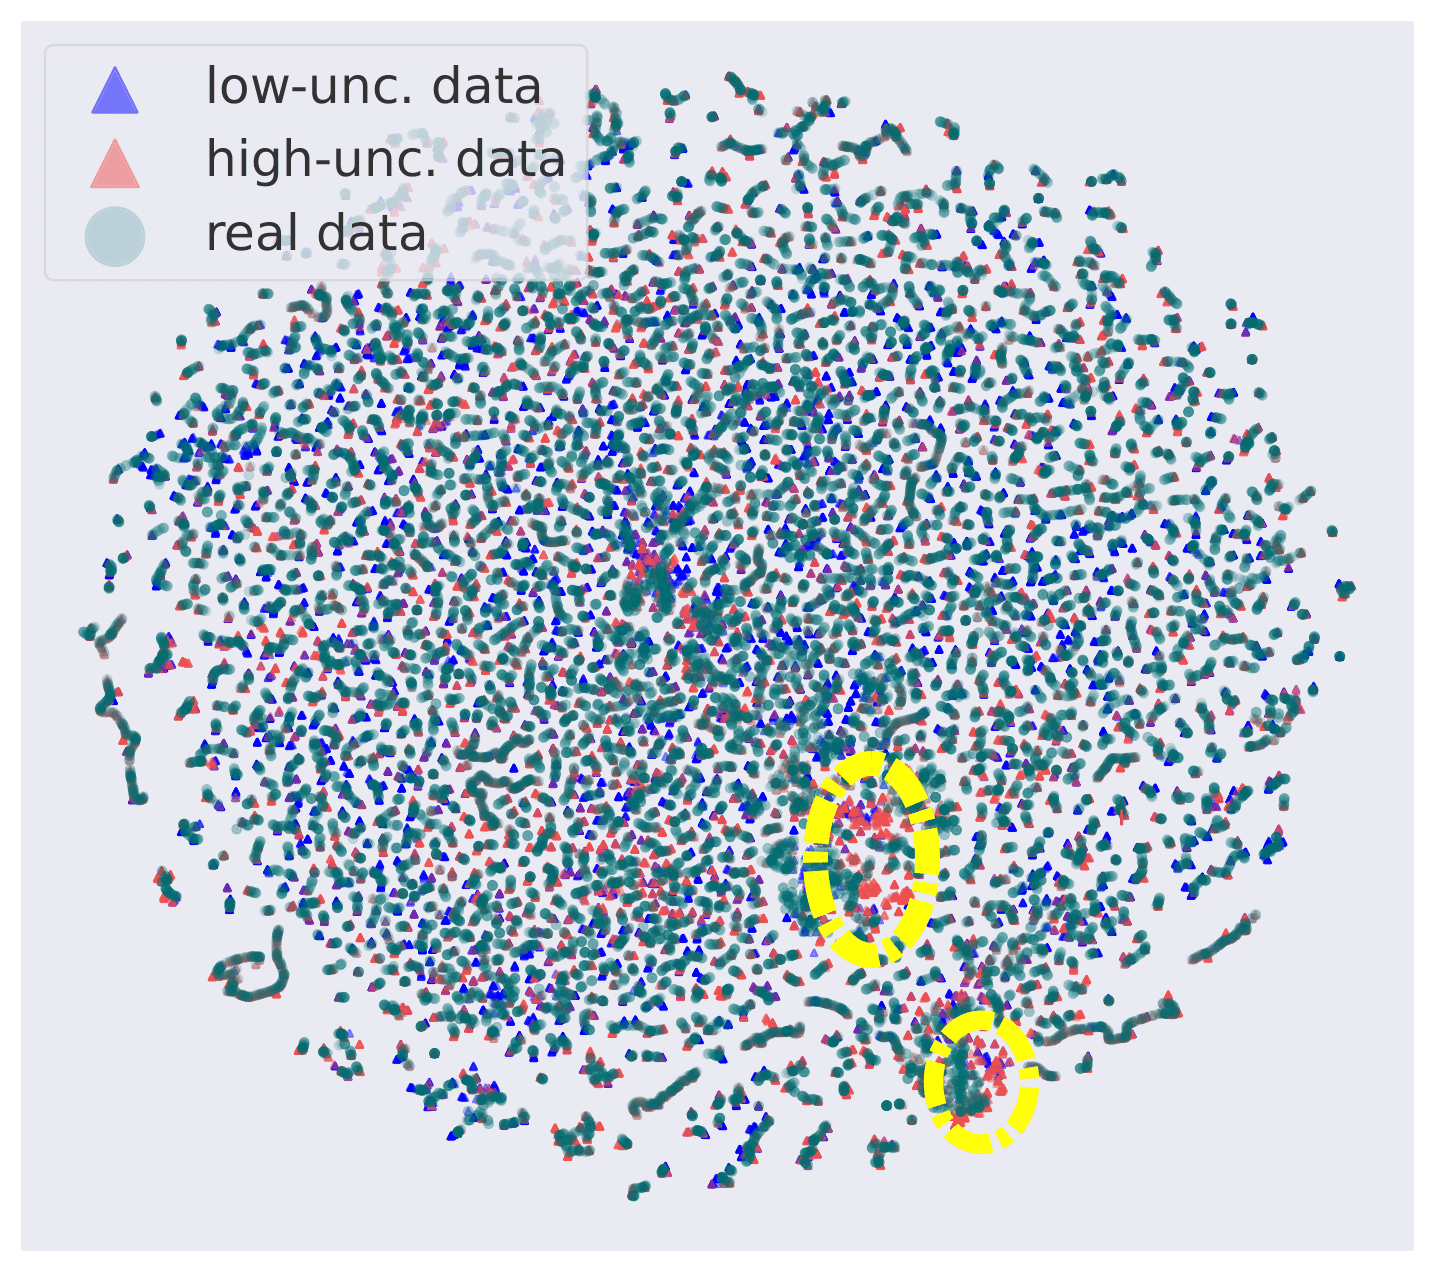
\includegraphics[width=0.95\linewidth]{fig/exp/tsne-1.png}
        \caption{Visualization of the projected distributions for real and imaginary datasets. }
        \label{fig:vis}
    \end{center}
    \vspace{-0.2cm}
\end{wrapfigure}
In this section, we visualize the imaginary dataset to analyze the quality of its generation and uncertainty estimation.  We choose t-SNE~\citep{mataten2008tsne} as the visualization method and project the imaginary dataset and a real dataset collected by the rule-based policy into 2-d space for comparison. The results are in Figure.~\ref{fig:vis}. The "real data" marks the data collected by the rule-based policy, while "low-unc. data" and "high-unc. data" represent segments of the imaginary dataset categorized by their uncertainty scores $R_\transf$ and $R_{\rewf}$ falling within the lower and upper 50\% percentiles, respectively. The real data and the imaginary data follow a similar data distribution, which indicates the effectiveness of the rehearsing process in \algo. Besides, as highlighted by the yellow dashed circles, the uncertainty score also identifies parts of the clusters that are out of the real data distribution, which will be penalized when introspecting via CIQL. The results give us more confidence about the effectiveness of the URI framework.

% Besides, we use t-SNE~\citep{mataten2008tsne} to project imaginary dataset and a real dataset collected by the rule-based policy for comparison, where the results are in Figure.~\ref{fig:vis}. The "real data" is collected by the rule-based policy, while "low-unc. data" and "high-unc. data" represent segments of the imaginary dataset categorized by their uncertainty scores $R_\transf$ and $R_{\rewf}$ falling within the lower and upper 50\% percentiles, respectively. It is easy to see that the real data and the imaginary dataset are overall in the same data distribution, which indicates the effectiveness of the rehearsing process in \algo. Besides, as highlighted by the yellow dashed circles, the uncertainty score also identifies parts of the clusters that are out of the real data distribution, which will be penalties when introspecting via CIQL. The results give us more confidence about the effectiveness of the URI framework.



% \begin{itemize}
%     % \item description of the implementation, how to select the start point, how to start and end.
%     \item vis the distribution of generated dataset and real dataset via some projection;
%     % \item Show one example of retrieval, Stage 1, Stage 2: given state, the find codes, stage-1 results, stage-2 results.
% \end{itemize}
